\hypertarget{sec-large-benchmarking}{%
\chapter{Large-Scale Benchmarking}\label{sec-large-benchmarking}}

\vspace{-15mm}\addtocontents{toc}{\textit{Sebastian Fischer, Michel Lang and Marc Becker}}

\textbf{Sebastian Fischer} \newline 
\emph{Ludwig-Maximilians-Universität München, and Munich Center for
Machine Learning (MCML)}

\textbf{Michel Lang} \newline  \emph{Research Center Trustworthy Data
Science and Security, and TU Dortmund University}

\textbf{Marc Becker} \newline  \emph{Ludwig-Maximilians-Universität
München, and Munich Center for Machine Learning (MCML)}
\newline \newline 

In machine learning, it is often difficult to evaluate methods using
mathematical analysis alone. Even when formal analyses can be
successfully applied, it is often an open question whether real-world
datasets satisfy the necessary assumptions for the theorems to hold.
Empirical benchmark experiments\index{benchmark experiments} evaluate
the performance of different algorithms on a wide range of datasets.
These empirical investigations are essential for understanding the
capabilities and limitations of existing methods and for developing new
and improved approaches. Trustworthy benchmark experiments are often
`large-scale', which means they may make use of many datasets, measures,
and learners. Moreover, datasets must span a wide range of domains and
problem types as conclusions can only be drawn about the kind of
datasets on which the benchmark
study\index{benchmark study|see{benchmark experiment}} was conducted.

Large-scale benchmark experiments consist of three primary steps:
sourcing the data for the experiment, executing the experiment, and
analyzing the results; we will discuss each of these in turn. In
Section~\ref{sec-openml} we will begin by discussing
\href{https://mlr3oml.mlr-org.com}{\texttt{mlr3oml}}, which provides an
interface between
\href{https://mlr3.mlr-org.com}{\texttt{mlr3}}\index{\texttt{mlr3}} and
OpenML (Vanschoren et al. 2013), a popular tool for uploading and
downloading datasets. Increasing the number of datasets leads to
`large-scale' experiments that may require significant computational
resources, so in Section~\ref{sec-hpc-exec} we will introduce
\href{https://mlr3batchmark.mlr-org.com}{\texttt{mlr3batchmark}}, which
connects \texttt{mlr3} with
\href{https://cran.r-project.org/package=batchtools}{\texttt{batchtools}}
(Lang, Bischl, and Surmann 2017), which provides methods for managing
and executing experiments on high-performance
computing\index{high-performance computing} (HPC) clusters. Finally, in
Section~\ref{sec-benchmark-analysis} we will demonstrate how to make use
of \href{https://mlr3benchmark.mlr-org.com}{\texttt{mlr3benchmark}} to
formally analyze the results from large-scale benchmark experiments.

Throughout this chapter, we will use the running example of benchmarking
a random forest model against a logistic regression as in Couronné,
Probst, and Boulesteix (2018). We will also assume that you have read
Chapter~\ref{sec-pipelines} and Chapter~\ref{sec-technical}. We make use
of \texttt{ppl("robustify")} (Section~\ref{sec-prepro-robustify}) for
automating common preprocessing steps. We also set a featureless
baseline as a fallback learner (Section~\ref{sec-fallback}) and set
\texttt{"try"} as our encapsulation method
(Section~\ref{sec-encapsulation}), which logs errors/warnings to an
external file that can be read by \texttt{batchtools} (we will return to
this in Section~\ref{sec-batchtools-monitoring}).

\begin{Shaded}
\begin{Highlighting}[]
\CommentTok{\# featureless baseline}
\NormalTok{lrn\_baseline }\OtherTok{=} \FunctionTok{lrn}\NormalTok{(}\StringTok{"classif.featureless"}\NormalTok{, }\AttributeTok{id =} \StringTok{"featureless"}\NormalTok{)}

\CommentTok{\# logistic regression pipeline}
\NormalTok{lrn\_lr }\OtherTok{=} \FunctionTok{lrn}\NormalTok{(}\StringTok{"classif.log\_reg"}\NormalTok{)}
\NormalTok{lrn\_lr }\OtherTok{=} \FunctionTok{as\_learner}\NormalTok{(}\FunctionTok{ppl}\NormalTok{(}\StringTok{"robustify"}\NormalTok{, }\AttributeTok{learner =}\NormalTok{ lrn\_lr) }\SpecialCharTok{\%\textgreater{}\textgreater{}\%}\NormalTok{ lrn\_lr)}
\NormalTok{lrn\_lr}\SpecialCharTok{$}\NormalTok{id }\OtherTok{=} \StringTok{"logreg"}
\NormalTok{lrn\_lr}\SpecialCharTok{$}\NormalTok{fallback }\OtherTok{=}\NormalTok{ lrn\_baseline}
\NormalTok{lrn\_lr}\SpecialCharTok{$}\NormalTok{encapsulate }\OtherTok{=} \FunctionTok{c}\NormalTok{(}\AttributeTok{train =} \StringTok{"try"}\NormalTok{, }\AttributeTok{predict =} \StringTok{"try"}\NormalTok{)}

\CommentTok{\# random forest pipeline}
\NormalTok{lrn\_rf }\OtherTok{=} \FunctionTok{lrn}\NormalTok{(}\StringTok{"classif.ranger"}\NormalTok{)}
\NormalTok{lrn\_rf }\OtherTok{=} \FunctionTok{as\_learner}\NormalTok{(}\FunctionTok{ppl}\NormalTok{(}\StringTok{"robustify"}\NormalTok{, }\AttributeTok{learner =}\NormalTok{ lrn\_rf) }\SpecialCharTok{\%\textgreater{}\textgreater{}\%}\NormalTok{ lrn\_rf)}
\NormalTok{lrn\_rf}\SpecialCharTok{$}\NormalTok{id }\OtherTok{=} \StringTok{"ranger"}
\NormalTok{lrn\_rf}\SpecialCharTok{$}\NormalTok{fallback }\OtherTok{=}\NormalTok{ lrn\_baseline}
\NormalTok{lrn\_rf}\SpecialCharTok{$}\NormalTok{encapsulate }\OtherTok{=} \FunctionTok{c}\NormalTok{(}\AttributeTok{train =} \StringTok{"try"}\NormalTok{, }\AttributeTok{predict =} \StringTok{"try"}\NormalTok{)}

\NormalTok{learners }\OtherTok{=} \FunctionTok{list}\NormalTok{(lrn\_lr, lrn\_rf, lrn\_baseline)}
\end{Highlighting}
\end{Shaded}

As a starting example, we will compare our learners across three
classification tasks using accuracy and three-fold CV.

\begin{Shaded}
\begin{Highlighting}[]
\NormalTok{design }\OtherTok{=} \FunctionTok{benchmark\_grid}\NormalTok{(}\FunctionTok{tsks}\NormalTok{(}\FunctionTok{c}\NormalTok{(}\StringTok{"german\_credit"}\NormalTok{, }\StringTok{"sonar"}\NormalTok{, }\StringTok{"pima"}\NormalTok{)),}
\NormalTok{  learners, }\FunctionTok{rsmp}\NormalTok{(}\StringTok{"cv"}\NormalTok{, }\AttributeTok{folds =} \DecValTok{10}\NormalTok{))}
\NormalTok{bmr }\OtherTok{=} \FunctionTok{benchmark}\NormalTok{(design)}
\NormalTok{bmr}\SpecialCharTok{$}\FunctionTok{aggregate}\NormalTok{(}\FunctionTok{msr}\NormalTok{(}\StringTok{"classif.acc"}\NormalTok{))[, .(task\_id, learner\_id, classif.acc)]}
\end{Highlighting}
\end{Shaded}

\begin{verbatim}
         task_id  learner_id classif.acc
1: german_credit      logreg      0.7460
2: german_credit      ranger      0.7610
3: german_credit featureless      0.7000
4:         sonar      logreg      0.7162
5:         sonar      ranger      0.8317
6:         sonar featureless      0.5329
7:          pima      logreg      0.7747
8:          pima      ranger      0.7683
9:          pima featureless      0.6511
\end{verbatim}

In this small experiment, random forests appears to outperform the other
learners on all three datasets. However, this analysis is not conclusive
as we only considered three tasks, and the performance differences might
not be statistically significant. In the following, we will introduce
some techniques to improve the study.

\hypertarget{sec-openml}{%
\section{Getting Data with OpenML}\label{sec-openml}}

To draw meaningful conclusions from benchmark experiments, a good choice
of datasets and tasks is essential.
OpenML\index{OpenML}{\marginnote{\begin{footnotesize}OpenML\end{footnotesize}}}
is an open-source platform that facilitates the sharing and
dissemination of machine learning research data, algorithms, and
experimental results, in a standardized format enabling consistent
cross-study comparison. OpenML's design ensures that all data on the
platform is `FAIR\index{FAIR}' (\textbf{F}indability,
\textbf{A}ccessibility, \textbf{I}nteroperability and
\textbf{R}eusability), which ensures the data is easily discoverable and
reusable. All entities on the platform have unique identifiers and
standardized (meta)data that can be accessed via a REST API or the web
interface.

In this section, we will cover some of the main features of OpenML and
how to use them via the
\href{https://mlr3oml.mlr-org.com}{\texttt{mlr3oml}}\index{\texttt{mlr3oml}}
interface package. In particular, we will discuss OpenML datasets,
tasks, and task collections, but will not cover algorithms or experiment
results here.

\hypertarget{sec-openml-dataset}{%
\subsection{Datasets}\label{sec-openml-dataset}}

Finding data from OpenML is possible via the website or its REST API
that \texttt{mlr3oml} interfaces.
\href{https://mlr3oml.mlr-org.com/reference/list_oml.html}{\texttt{list\_oml\_data()}}
can be used to filter datasets for specific properties, for example by
number of features, rows, or number of classes in a classification
problem:

\begin{Shaded}
\begin{Highlighting}[]
\FunctionTok{library}\NormalTok{(mlr3oml)}

\NormalTok{odatasets }\OtherTok{=} \FunctionTok{list\_oml\_data}\NormalTok{(}
  \AttributeTok{number\_features =} \FunctionTok{c}\NormalTok{(}\DecValTok{10}\NormalTok{, }\DecValTok{20}\NormalTok{),}
  \AttributeTok{number\_instances =} \FunctionTok{c}\NormalTok{(}\DecValTok{45000}\NormalTok{, }\DecValTok{50000}\NormalTok{),}
  \AttributeTok{number\_classes =} \DecValTok{2}
\NormalTok{)}
\end{Highlighting}
\end{Shaded}

\begin{Shaded}
\begin{Highlighting}[]
\NormalTok{odatasets[NumberOfFeatures }\SpecialCharTok{\textless{}} \DecValTok{16}\NormalTok{,}
  \FunctionTok{c}\NormalTok{(}\StringTok{"data\_id"}\NormalTok{, }\StringTok{"name"}\NormalTok{, }\StringTok{"NumberOfFeatures"}\NormalTok{, }\StringTok{"NumberOfInstances"}\NormalTok{)]}
\end{Highlighting}
\end{Shaded}

\begin{verbatim}
   data_id       name NumberOfFeatures NumberOfInstances
1:     179      adult               15             48842
2:    1590      adult               15             48842
3:   43898      adult               15             48790
4:   45051 adult-test               15             48842
5:   45068      adult               15             48842
\end{verbatim}

Note that \texttt{list\_oml\_data()} returns a \texttt{data.table} with
many more meta-features than shown here; this table can itself be used
to filter further.

We can see that some datasets have duplicated names, which is why each
dataset also has a unique ID. By example, let us consider the `adult'
dataset with ID 1590. Metadata for the dataset is loaded with
\href{https://mlr3oml.mlr-org.com/reference/oml_sugar.html}{\texttt{odt()}}\index{\texttt{odt()}}{\marginnote{\begin{footnotesize}\texttt{odt()}\end{footnotesize}}},
which returns an object of class
\href{https://mlr3oml.mlr-org.com/reference/oml_data.html}{\texttt{OMLData}}.

\begin{Shaded}
\begin{Highlighting}[]
\NormalTok{odata }\OtherTok{=} \FunctionTok{odt}\NormalTok{(}\AttributeTok{id =} \DecValTok{1590}\NormalTok{)}
\NormalTok{odata}
\end{Highlighting}
\end{Shaded}

\begin{verbatim}
<OMLData:1590:adult> (48842x15)
 * Default target: class
\end{verbatim}

The \texttt{OMLData} object contains metadata about the dataset but
importantly does not (yet) contain the data. This means that information
about the dataset can be queried without having to load the entire data
into memory, for example, the license and dimension of the data:

\begin{Shaded}
\begin{Highlighting}[]
\NormalTok{odata}\SpecialCharTok{$}\NormalTok{license}
\end{Highlighting}
\end{Shaded}

\begin{verbatim}
[1] "Public"
\end{verbatim}

\begin{Shaded}
\begin{Highlighting}[]
\FunctionTok{c}\NormalTok{(}\AttributeTok{nrow =}\NormalTok{ odata}\SpecialCharTok{$}\NormalTok{nrow, }\AttributeTok{ncol =}\NormalTok{ odata}\SpecialCharTok{$}\NormalTok{ncol)}
\end{Highlighting}
\end{Shaded}

\begin{verbatim}
 nrow  ncol 
48842    15 
\end{verbatim}

If we want to work with the actual data, then accessing the
\texttt{\$data} field will download the data, import it into R, and then
store the \texttt{data.frame} in the \texttt{OMLData} object:

\begin{Shaded}
\begin{Highlighting}[]
\CommentTok{\# first 5 rows and columns}
\NormalTok{odata}\SpecialCharTok{$}\NormalTok{data[}\DecValTok{1}\SpecialCharTok{:}\DecValTok{5}\NormalTok{, }\DecValTok{1}\SpecialCharTok{:}\DecValTok{5}\NormalTok{]}
\end{Highlighting}
\end{Shaded}

\begin{verbatim}
   age workclass fnlwgt    education education.num
1:  25   Private 226802         11th             7
2:  38   Private  89814      HS-grad             9
3:  28 Local-gov 336951   Assoc-acdm            12
4:  44   Private 160323 Some-college            10
5:  18      <NA> 103497 Some-college            10
\end{verbatim}

\begin{tcolorbox}[enhanced jigsaw, opacitybacktitle=0.6, rightrule=.15mm, opacityback=0, arc=.35mm, breakable, titlerule=0mm, colframe=quarto-callout-tip-color-frame, coltitle=black, bottomrule=.15mm, toprule=.15mm, colback=white, colbacktitle=quarto-callout-tip-color!10!white, bottomtitle=1mm, toptitle=1mm, title=\textcolor{quarto-callout-tip-color}{\faLightbulb}\hspace{0.5em}{mlr3oml Cache}, leftrule=.75mm, left=2mm]

After \texttt{\$data} has been called the first time, all subsequent
calls to \texttt{\$data} will be transparently redirected to the
in-memory \texttt{data.frame}. Additionally, many objects can be
permanently cached on the local file system by setting the option
\texttt{mlr3oml.cache} to either \texttt{TRUE} or to a specific path to
be used as the cache folder.

\end{tcolorbox}

Data can then be converted into \texttt{mlr3} backends (see
Section~\ref{sec-backends}) with the
\href{https://mlr3.mlr-org.com/reference/as_data_backend.Matrix.html}{\texttt{as\_data\_backend()}}
function and then into tasks:

\begin{Shaded}
\begin{Highlighting}[]
\NormalTok{backend }\OtherTok{=} \FunctionTok{as\_data\_backend}\NormalTok{(odata)}
\NormalTok{tsk\_adult }\OtherTok{=} \FunctionTok{as\_task\_classif}\NormalTok{(backend, }\AttributeTok{target =} \StringTok{"class"}\NormalTok{)}
\NormalTok{tsk\_adult}
\end{Highlighting}
\end{Shaded}

\begin{verbatim}
<TaskClassif:backend> (48842 x 15)
* Target: class
* Properties: twoclass
* Features (14):
  - fct (8): education, marital.status, native.country,
    occupation, race, relationship, sex, workclass
  - int (6): age, capital.gain, capital.loss, education.num,
    fnlwgt, hours.per.week
\end{verbatim}

Some datasets on OpenML contain columns that should neither be used as a
feature nor a target. The column names that are usually included as
features are accessible through the field \texttt{\$feature\_names}, and
we assign them to the \texttt{mlr3} task accordingly. Note that for the
dataset at hand, this would not have been necessary, as all non-target
columns are to be treated as predictors, but we include it for clarity.

\begin{Shaded}
\begin{Highlighting}[]
\NormalTok{tsk\_adult}\SpecialCharTok{$}\NormalTok{col\_roles}\SpecialCharTok{$}\NormalTok{feature }\OtherTok{=}\NormalTok{ odata}\SpecialCharTok{$}\NormalTok{feature\_names}
\NormalTok{tsk\_adult}
\end{Highlighting}
\end{Shaded}

\begin{verbatim}
<TaskClassif:backend> (48842 x 15)
* Target: class
* Properties: twoclass
* Features (14):
  - fct (8): education, marital.status, native.country,
    occupation, race, relationship, sex, workclass
  - int (6): age, capital.gain, capital.loss, education.num,
    fnlwgt, hours.per.week
\end{verbatim}

\hypertarget{sec-openml-task}{%
\subsection{Task}\label{sec-openml-task}}

OpenML tasks are built on top of OpenML datasets and additionally
specify the target variable, the train-test splits to use for
resampling, and more. Note that this differs from \texttt{mlr3}
\texttt{Task} objects, which do not contain information about the
resampling procedure. Similarly to \texttt{mlr3}, OpenML has different
types of tasks, such as regression and classification. Analogously to
filtering datasets, tasks can be filtered with
\href{https://mlr3oml.mlr-org.com/reference/list_oml.html}{\texttt{list\_oml\_tasks()}}.
To find a task that makes use of the data we have been using, we would
pass the data ID to the \texttt{data\_id} argument:

\begin{Shaded}
\begin{Highlighting}[]
\CommentTok{\# tasks making use of the adult data}
\NormalTok{adult\_tasks }\OtherTok{=} \FunctionTok{list\_oml\_tasks}\NormalTok{(}\AttributeTok{data\_id =} \DecValTok{1590}\NormalTok{)}
\end{Highlighting}
\end{Shaded}

\begin{Shaded}
\begin{Highlighting}[]
\NormalTok{adult\_tasks[task\_type }\SpecialCharTok{==} \StringTok{"Supervised Classification"}\NormalTok{, task\_id]}
\end{Highlighting}
\end{Shaded}

\begin{verbatim}
[1]   7592  14947 126025 146154 146598 168878 233099 359983 361515
\end{verbatim}

From these tasks, we randomly select the task with ID 359983. We can
load the object using
\href{https://mlr3oml.mlr-org.com/reference/oml_sugar.html}{\texttt{otsk()}}\index{\texttt{otsk()}}{\marginnote{\begin{footnotesize}\texttt{otsk()}\end{footnotesize}}},
which returns an
\href{https://mlr3oml.mlr-org.com/reference/oml_task.html}{\texttt{OMLTask}}
object.

\begin{Shaded}
\begin{Highlighting}[]
\NormalTok{otask }\OtherTok{=} \FunctionTok{otsk}\NormalTok{(}\AttributeTok{id =} \DecValTok{359983}\NormalTok{)}
\NormalTok{otask}
\end{Highlighting}
\end{Shaded}

\begin{verbatim}
<OMLTask:359983>
 * Type: Supervised Classification
 * Data: adult (id: 1590; dim: 48842x15)
 * Target: class
 * Estimation: crossvalidation (id: 1; repeats: 1, folds: 10)
\end{verbatim}

The \texttt{OMLData} object associated with the underlying dataset can
be accessed through the \texttt{\$data} field.

\begin{Shaded}
\begin{Highlighting}[]
\NormalTok{otask}\SpecialCharTok{$}\NormalTok{data}
\end{Highlighting}
\end{Shaded}

\begin{verbatim}
<OMLData:1590:adult> (48842x15)
 * Default target: class
\end{verbatim}

The data splits associated with the estimation procedure are accessible
through the field \texttt{\$task\_splits}. In \texttt{mlr3} terms, these
are the instantiation of a
\href{https://mlr3.mlr-org.com/reference/Resampling.html}{\texttt{Resampling}}
on a specific
\href{https://mlr3.mlr-org.com/reference/Task.html}{\texttt{Task}}.

\begin{Shaded}
\begin{Highlighting}[]
\NormalTok{otask}\SpecialCharTok{$}\NormalTok{task\_splits}
\end{Highlighting}
\end{Shaded}

\begin{verbatim}
         type rowid repeat. fold
     1: TRAIN 32427       0    0
     2: TRAIN 13077       0    0
     3: TRAIN 15902       0    0
     4: TRAIN 17703       0    0
     5: TRAIN 35511       0    0
    ---                         
488416:  TEST  8048       0    9
488417:  TEST 12667       0    9
488418:  TEST 43944       0    9
488419:  TEST 25263       0    9
488420:  TEST 43381       0    9
\end{verbatim}

The OpenML task can be converted to both an \texttt{mlr3::Task} and
\href{https://mlr3.mlr-org.com/reference/ResamplingCustom.html}{\texttt{ResamplingCustom}}
instantiated on the task using
\href{https://mlr3.mlr-org.com/reference/as_task.html}{\texttt{as\_task()}}
and
\href{https://mlr3.mlr-org.com/reference/as_resampling.html}{\texttt{as\_resampling()}},
respectively:

\begin{Shaded}
\begin{Highlighting}[]
\NormalTok{tsk\_adult }\OtherTok{=} \FunctionTok{as\_task}\NormalTok{(otask)}
\NormalTok{tsk\_adult}
\end{Highlighting}
\end{Shaded}

\begin{verbatim}
<TaskClassif:adult> (48842 x 15)
* Target: class
* Properties: twoclass
* Features (14):
  - fct (8): education, marital.status, native.country,
    occupation, race, relationship, sex, workclass
  - int (6): age, capital.gain, capital.loss, education.num,
    fnlwgt, hours.per.week
\end{verbatim}

\begin{Shaded}
\begin{Highlighting}[]
\NormalTok{resampling }\OtherTok{=} \FunctionTok{as\_resampling}\NormalTok{(otask)}
\NormalTok{resampling}
\end{Highlighting}
\end{Shaded}

\begin{verbatim}
<ResamplingCustom>: Custom Splits
* Iterations: 10
* Instantiated: TRUE
* Parameters: list()
\end{verbatim}

\texttt{mlr3oml} also allows direct construction of \texttt{mlr3} tasks
and resamplings with the standard
\href{https://mlr3.mlr-org.com/reference/mlr_sugar.html}{\texttt{tsk()}}
and
\href{https://mlr3.mlr-org.com/reference/mlr_sugar.html}{\texttt{rsmp()}}
constructors, e.g.:

\begin{Shaded}
\begin{Highlighting}[]
\FunctionTok{tsk}\NormalTok{(}\StringTok{"oml"}\NormalTok{, }\AttributeTok{task\_id =} \DecValTok{359983}\NormalTok{)}
\end{Highlighting}
\end{Shaded}

\begin{verbatim}
<TaskClassif:adult> (48842 x 15)
* Target: class
* Properties: twoclass
* Features (14):
  - fct (8): education, marital.status, native.country,
    occupation, race, relationship, sex, workclass
  - int (6): age, capital.gain, capital.loss, education.num,
    fnlwgt, hours.per.week
\end{verbatim}

\hypertarget{sec-openml-collection}{%
\subsection{Task Collection}\label{sec-openml-collection}}

The OpenML task collection is a container object bundling existing
tasks. This allows for the creation of benchmark
suites\index{benchmark suites}, which are curated collections of tasks
that satisfy certain quality criteria. Examples include the OpenML CC-18
benchmark suite (Bischl et al. 2021), the AutoML benchmark (Gijsbers et
al. 2022) and the benchmark for tabular deep learning (Grinsztajn,
Oyallon, and Varoquaux 2022).
\href{https://mlr3oml.mlr-org.com/reference/oml_collection.html}{\texttt{OMLCollection}}
objects are loaded with
\href{https://mlr3oml.mlr-org.com/reference/oml_sugar.html}{\texttt{ocl()}}\index{\texttt{ocl()}}{\marginnote{\begin{footnotesize}\texttt{ocl()}\end{footnotesize}}},
by example we will look at CC-18, which has ID 99:

\begin{Shaded}
\begin{Highlighting}[]
\NormalTok{otask\_collection }\OtherTok{=} \FunctionTok{ocl}\NormalTok{(}\AttributeTok{id =} \DecValTok{99}\NormalTok{)}
\end{Highlighting}
\end{Shaded}

\begin{Shaded}
\begin{Highlighting}[]
\NormalTok{otask\_collection}
\end{Highlighting}
\end{Shaded}

\begin{verbatim}
<OMLCollection: 99> OpenML-CC18 Curated Class[...]
 * data:  72
 * tasks: 72
\end{verbatim}

The task includes 72 classification tasks on different datasets that can
be accessed through \texttt{\$task\_ids}:

\begin{Shaded}
\begin{Highlighting}[]
\NormalTok{otask\_collection}\SpecialCharTok{$}\NormalTok{task\_ids[}\DecValTok{1}\SpecialCharTok{:}\DecValTok{5}\NormalTok{] }\CommentTok{\# first 5 tasks in the collection}
\end{Highlighting}
\end{Shaded}

\begin{verbatim}
[1]  3  6 11 12 14
\end{verbatim}

Task collections can be used to quickly define benchmark experiments in
\texttt{mlr3}. To easily construct all tasks and resamplings from the
benchmarking suite, you can use
\href{https://mlr3.mlr-org.com/reference/as_task.html}{\texttt{as\_tasks()}}\index{\texttt{as\_tasks()}}
and
\href{https://mlr3.mlr-org.com/reference/as_resampling.html}{\texttt{as\_resamplings()}}\index{\texttt{as\_resamplings()}}
respectively:

\begin{Shaded}
\begin{Highlighting}[]
\NormalTok{tasks }\OtherTok{=} \FunctionTok{as\_tasks}\NormalTok{(otask\_collection)}
\NormalTok{resamplings }\OtherTok{=} \FunctionTok{as\_resamplings}\NormalTok{(otask\_collection)}
\end{Highlighting}
\end{Shaded}

Alternatively, if we wanted to filter the collection further, say to a
binary classification experiment with six tasks, we could run
\href{https://mlr3oml.mlr-org.com/reference/list_oml.html}{\texttt{list\_oml\_tasks()}}
with the task IDs from the CC-18 collection as argument
\texttt{task\_id}. We can either use the \texttt{list\_oml\_tasks()}
argument to request the number of classes to be \texttt{2}, or we can
make use of the fact that the result of \texttt{list\_oml\_tasks()} is a
\texttt{data.table} and subset the resulting table.

\begin{Shaded}
\begin{Highlighting}[]
\NormalTok{binary\_cc18 }\OtherTok{=} \FunctionTok{list\_oml\_tasks}\NormalTok{(}
  \AttributeTok{limit =} \DecValTok{6}\NormalTok{,}
  \AttributeTok{task\_id =}\NormalTok{ otask\_collection}\SpecialCharTok{$}\NormalTok{task\_ids,}
  \AttributeTok{number\_classes =} \DecValTok{2}
\NormalTok{)}
\end{Highlighting}
\end{Shaded}

We now define the tasks and resamplings which we will use for comparing
the logistic regression with the random forest learner. Note that all
resamplings in this collection consist of exactly 10 iterations.

\begin{Shaded}
\begin{Highlighting}[]
\CommentTok{\# load tasks as a list}
\NormalTok{otasks }\OtherTok{=} \FunctionTok{lapply}\NormalTok{(binary\_cc18}\SpecialCharTok{$}\NormalTok{task\_id, otsk)}

\CommentTok{\# convert to mlr3 tasks and resamplings}
\NormalTok{tasks }\OtherTok{=} \FunctionTok{as\_tasks}\NormalTok{(otasks)}
\NormalTok{resamplings }\OtherTok{=} \FunctionTok{as\_resamplings}\NormalTok{(otasks)}
\end{Highlighting}
\end{Shaded}

To define the design table, we use
\href{https://mlr3.mlr-org.com/reference/benchmark_grid.html}{\texttt{benchmark\_grid()}}
and set \texttt{paired} to \texttt{TRUE}, which is used in situations
where each resampling is instantiated on a corresponding task (therefore
the \texttt{tasks} and \texttt{resamplings} below must have the same
length) and each learner should be evaluated on every resampled task.

\begin{Shaded}
\begin{Highlighting}[]
\NormalTok{large\_design }\OtherTok{=} \FunctionTok{benchmark\_grid}\NormalTok{(tasks, learners, resamplings,}
  \AttributeTok{paired =} \ConstantTok{TRUE}\NormalTok{)}
\NormalTok{large\_design[}\DecValTok{1}\SpecialCharTok{:}\DecValTok{6}\NormalTok{] }\CommentTok{\# first 6 rows}
\end{Highlighting}
\end{Shaded}

\begin{verbatim}
       task     learner resampling
1: kr-vs-kp      logreg     custom
2: kr-vs-kp      ranger     custom
3: kr-vs-kp featureless     custom
4: breast-w      logreg     custom
5: breast-w      ranger     custom
6: breast-w featureless     custom
\end{verbatim}

Having set up our large experiment, we can now look at how to
efficiently carry it out on a cluster.

\hypertarget{sec-hpc-exec}{%
\section{Benchmarking on HPC Clusters}\label{sec-hpc-exec}}

As discussed in Section~\ref{sec-parallelization}, parallelization of
benchmark experiments is straightforward as they are embarrassingly
parallel\index{embarrassingly parallel}. However, for large experiments,
parallelization on a high-performance
computing\index{high-performance computing}{\marginnote{\begin{footnotesize}High-performance
Computing\end{footnotesize}}} (HPC) cluster is often preferable.
\href{https://cran.r-project.org/package=batchtools}{\texttt{batchtools}}
provides a framework to simplify running large batches of computational
experiments in parallel from R on such sites. It is highly flexible,
making it suitable for a wide range of computational experiments,
including machine learning, optimization, simulation, and more.

\begin{tcolorbox}[enhanced jigsaw, opacitybacktitle=0.6, rightrule=.15mm, opacityback=0, arc=.35mm, breakable, titlerule=0mm, colframe=quarto-callout-tip-color-frame, coltitle=black, bottomrule=.15mm, toprule=.15mm, colback=white, colbacktitle=quarto-callout-tip-color!10!white, bottomtitle=1mm, toptitle=1mm, title=\textcolor{quarto-callout-tip-color}{\faLightbulb}\hspace{0.5em}{\texttt{"batchtools"} backend for \texttt{future}}, leftrule=.75mm, left=2mm]

In Section~\ref{sec-parallel-resample} we touched upon different
parallelization backends. The package
\href{https://cran.r-project.org/package=future}{\texttt{future}}
includes a \texttt{"batchtools"} plan, however, this does not allow the
additional control that comes with working with \texttt{batchtools}
directly.

\end{tcolorbox}

An HPC cluster is a collection of interconnected computers or servers
providing computational power beyond what a single computer can achieve.
HPC clusters typically consist of multiple compute nodes, each with
multiple CPU/GPU cores, memory, and local storage. These nodes are
usually connected by a high-speed network and network file system which
enables the nodes to communicate and work together on a given task. The
most important difference between HPC clusters and a personal computer
(PC), is that the nodes often cannot be accessed directly, but instead,
computational jobs are queued by a scheduling
system\index{scheduling system} such as Slurm (Simple Linux Utility for
Resource Management). A scheduling system is a software tool that
orchestrates the allocation of computing resources to users or
applications on the cluster. It ensures that multiple users and
applications can access the resources of the cluster fairly and
efficiently, and also helps to maximize the utilization of the computing
resources.

Figure~\ref{fig-hpc} contains a rough sketch of an HPC architecture.
Multiple users can log into the head node (typically via SSH) and add
their computational job\index{computational job}s to the queue by
sending a command of the form ``execute computation X using resources Y
for Z amount of time''. The scheduling system controls when these
computational jobs are executed.

For the rest of this section, we will look at how to use
\texttt{batchtools} and
\href{https://mlr3batchmark.mlr-org.com}{\texttt{mlr3batchmark}}\index{\texttt{mlr3batchmark}}
for submitting jobs, adapting jobs to clusters, ensuring
reproducibility, querying job status, and debugging failures.

\begin{figure}

{\centering 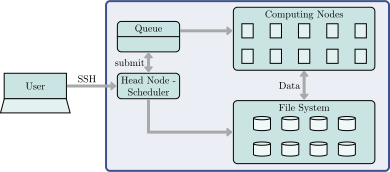
\includegraphics[width=1\textwidth,height=\textheight]{chapters/chapter11/Figures/mlr3book_figures-32.png}

}

\caption{\label{fig-hpc}Illustration of an HPC cluster architecture.}

\end{figure}

\hypertarget{sec-registry}{%
\subsection{Experiment Registry Setup}\label{sec-registry}}

\texttt{batchtools}\index{\texttt{batchtools}} is built around
experiments or `jobs\index{jobs}'. One replication of a job is defined
by applying a (parameterized) algorithm to a (parameterized) problem. A
benchmark experiment in \texttt{batchtools} consists of running many
such experiments with different algorithms, algorithm parameters,
problems, and problem parameters. Each such experiment is
computationally independent of all other experiments and constitutes the
basic level of computation \texttt{batchtools} can parallelize. For this
section, we will define a single \texttt{batchtools} experiment as one
resampling iteration of one learner on one task, in
Section~\ref{sec-custom-experiments} we will look at different ways of
defining an experiment.

The first step in running an experiment is to create or load an
experiment registry with
\href{https://www.rdocumentation.org/packages/batchtools/topics/makeExperimentRegistry}{\texttt{makeExperimentRegistry()}}
or
\href{https://www.rdocumentation.org/packages/batchtools/topics/loadRegistry}{\texttt{loadRegistry()}}
respectively. This constructs the inter-communication object for all
functions in \texttt{batchtools} and corresponds to a folder on the file
system. Among other things, the experiment registry stores the
algorithms, problems, and job definitions; log outputs and status of
submitted, running, and finished jobs; job results; and the ``cluster
function'' that defines the interaction with the scheduling system in a
scheduling-software-agnostic way.

Below, we create a registry in a subdirectory of our working directory
-- on a real cluster, make sure that this folder is stored on a shared
network filesystem, otherwise, the nodes cannot access it. We also set
the registry's \texttt{seed} to \texttt{1} and the \texttt{packages} to
\texttt{"mlr3verse"}, which will make these packages available in all
our experiments.

\begin{Shaded}
\begin{Highlighting}[]
\FunctionTok{library}\NormalTok{(batchtools)}

\CommentTok{\# create registry}
\NormalTok{reg }\OtherTok{=} \FunctionTok{makeExperimentRegistry}\NormalTok{(}
  \AttributeTok{file.dir =} \StringTok{"./experiments"}\NormalTok{,}
  \AttributeTok{seed =} \DecValTok{1}\NormalTok{,}
  \AttributeTok{packages =} \StringTok{"mlr3verse"}
\NormalTok{)}
\end{Highlighting}
\end{Shaded}

Once the registry has been created, we need to populate it with problems
and algorithms to form the jobs, this is most easily carried out with
\texttt{mlr3batchmark}\index{\texttt{mlr3batchmark}}, although finer
control is possible with \texttt{batchtools} and will be explored in
Section~\ref{sec-custom-experiments}.
\href{https://mlr3batchmark.mlr-org.com/reference/batchmark.html}{\texttt{batchmark()}}\index{\texttt{batchmark()}}
converts \texttt{mlr3} tasks and resamplings to \texttt{batchtools}
problems, and converts \texttt{mlr3} learners to \texttt{batchtools}
algorithms; jobs are then created for all resampling iterations.

\begin{Shaded}
\begin{Highlighting}[]
\FunctionTok{library}\NormalTok{(mlr3batchmark)}
\FunctionTok{batchmark}\NormalTok{(large\_design, }\AttributeTok{reg =}\NormalTok{ reg)}
\end{Highlighting}
\end{Shaded}

Now the registry includes six problems, one for each resampled task, and
\(180\) jobs from \(3\) learners \(\times\) \(6\) tasks \(\times\)
\(10\) resampling iterations. The single algorithm in the registry is
because \texttt{mlr3batchmark} specifies a single algorithm that is
parametrized with the learner IDs.

\begin{Shaded}
\begin{Highlighting}[]
\NormalTok{reg}
\end{Highlighting}
\end{Shaded}

\begin{verbatim}
Experiment Registry
  Backend   : Interactive
  File dir  : /your_directory/experiments
  Work dir  : /your_directory
  Jobs      : 180
  Problems  : 6
  Algorithms: 1
  Seed      : 1
  Writeable : TRUE
\end{verbatim}

By default, the ``Interactive'' cluster function (see
\href{https://www.rdocumentation.org/packages/batchtools/topics/makeClusterFunctionsInteractive}{\texttt{makeClusterFunctionsInteractive()}})
is used -- this is the abstraction for the scheduling system, and
``interactive'' here means to not use a real scheduler but instead to
use the interactive R session for sequential computation.
\href{https://www.rdocumentation.org/packages/batchtools/topics/getJobTable}{\texttt{getJobTable()}}
can be used to get more detailed information about the jobs. Here, we
only show a few selected columns for readability and unpack the list
columns \texttt{algo.pars} and \texttt{prob.pars} using
\href{https://www.rdocumentation.org/packages/batchtools/topics/unwrap}{\texttt{unwrap()}}.

\begin{Shaded}
\begin{Highlighting}[]
\NormalTok{job\_table }\OtherTok{=} \FunctionTok{getJobTable}\NormalTok{(}\AttributeTok{reg =}\NormalTok{ reg)}
\NormalTok{job\_table }\OtherTok{=} \FunctionTok{unwrap}\NormalTok{(job\_table)}
\NormalTok{job\_table }\OtherTok{=}\NormalTok{ job\_table[,}
\NormalTok{  .(job.id, learner\_id, task\_id, resampling\_id, repl)}
\NormalTok{]}

\NormalTok{job\_table}
\end{Highlighting}
\end{Shaded}

\begin{verbatim}
     job.id  learner_id  task_id resampling_id repl
  1:      1      logreg kr-vs-kp        custom    1
  2:      2      logreg kr-vs-kp        custom    2
  3:      3      logreg kr-vs-kp        custom    3
  4:      4      logreg kr-vs-kp        custom    4
  5:      5      logreg kr-vs-kp        custom    5
 ---                                               
176:    176 featureless spambase        custom    6
177:    177 featureless spambase        custom    7
178:    178 featureless spambase        custom    8
179:    179 featureless spambase        custom    9
180:    180 featureless spambase        custom   10
\end{verbatim}

In this output, we can see how each job is now assigned a unique
\texttt{job.id} and that each row corresponds to a single iteration
(column \texttt{repl}) of a resample experiment.

\hypertarget{sec-batchtools-submission}{%
\subsection{Job Submission}\label{sec-batchtools-submission}}

With the experiments defined, we can now submit them to the cluster.
However, it is best practice to first test each algorithm individually
using
\href{https://www.rdocumentation.org/packages/batchtools/topics/testJob}{\texttt{testJob()}}\index{\texttt{testJob()}}{\marginnote{\begin{footnotesize}\texttt{testJob()}\end{footnotesize}}}.
By example, we will only test the first job (\texttt{id\ =\ 1}) and will
use an external R session (\texttt{external\ =\ TRUE}).

\begin{Shaded}
\begin{Highlighting}[]
\NormalTok{result }\OtherTok{=} \FunctionTok{testJob}\NormalTok{(}\DecValTok{1}\NormalTok{, }\AttributeTok{external =} \ConstantTok{TRUE}\NormalTok{, }\AttributeTok{reg =}\NormalTok{ reg)}
\end{Highlighting}
\end{Shaded}

Once we are confident that the jobs are defined correctly (see
Section~\ref{sec-batchtools-monitoring} for jobs with errors), we can
proceed with their submission, by specifying the resource requirements
for each computational job and then optionally grouping jobs.

Configuration of resources is dependent on the cluster function set in
the registry. We will assume we are working with a Slurm\index{Slurm}
cluster and accordingly initialize the cluster function with
\href{https://www.rdocumentation.org/packages/batchtools/topics/makeClusterFunctionsSlurm}{\texttt{makeClusterFunctionsSlurm()}}
and will make use of the \texttt{slurm-simple.tml} template file that
can be found in a subdirectory of the \texttt{batchtools} package itself
(the exact location can be found by running
\texttt{system.file("templates",\ package\ =\ "batchtools")}), or the
\texttt{batchtools} GitHub repository. A template file is a shell script
with placeholders filled in by \texttt{batchtools} and contains the
command to start the computation via \texttt{Rscript} or
\texttt{R\ CMD\ batch}, as well as comments which serve as annotations
for the scheduler, for example, to communicate resources or paths on the
file system.

The exemplary template should work on many Slurm installations
out-of-the-box, but you might have to modify it for your cluster -- it
can be customized to work with more advanced configurations.

\begin{Shaded}
\begin{Highlighting}[]
\NormalTok{cf }\OtherTok{=} \FunctionTok{makeClusterFunctionsSlurm}\NormalTok{(}\AttributeTok{template =} \StringTok{"slurm{-}simple"}\NormalTok{)}
\end{Highlighting}
\end{Shaded}

To proceed with the examples on a local machine, we recommend setting
the cluster function to a Socket backend with
\href{https://www.rdocumentation.org/packages/batchtools/topics/makeClusterFunctionsSocket}{\texttt{makeClusterFunctionsSocket()}}.
The chosen cluster function can be saved to the registry by passing it
to the \texttt{\$cluster.functions} field.

\begin{Shaded}
\begin{Highlighting}[]
\NormalTok{reg}\SpecialCharTok{$}\NormalTok{cluster.functions }\OtherTok{=}\NormalTok{ cf}
\FunctionTok{saveRegistry}\NormalTok{(}\AttributeTok{reg =}\NormalTok{ reg)}
\end{Highlighting}
\end{Shaded}

With the registry setup, we can now decide if we want to run the
experiments in chunks (Section~\ref{sec-parallelization}) and then
specify the resource requirements for the submitted jobs.

For this example, we will use
\href{https://www.rdocumentation.org/packages/batchtools/topics/chunk}{\texttt{chunk()}}\index{\texttt{chunk()}}{\marginnote{\begin{footnotesize}\texttt{chunk()}\end{footnotesize}}}
to chunk\index{chunk} the jobs such that five iterations of one resample
experiment are run sequentially in one computational job -- in practice
the optimal grouping will be highly dependent on your experiment
(Section~\ref{sec-parallelization}).

\begin{Shaded}
\begin{Highlighting}[]
\NormalTok{ids }\OtherTok{=}\NormalTok{ job\_table}\SpecialCharTok{$}\NormalTok{job.id}
\NormalTok{chunks }\OtherTok{=} \FunctionTok{data.table}\NormalTok{(}
  \AttributeTok{job.id =}\NormalTok{ ids, }\AttributeTok{chunk =} \FunctionTok{chunk}\NormalTok{(ids, }\AttributeTok{chunk.size =} \DecValTok{5}\NormalTok{, }\AttributeTok{shuffle =} \ConstantTok{FALSE}\NormalTok{)}
\NormalTok{)}
\NormalTok{chunks[}\DecValTok{1}\SpecialCharTok{:}\DecValTok{6}\NormalTok{] }\CommentTok{\# first 6 jobs}
\end{Highlighting}
\end{Shaded}

\begin{verbatim}
   job.id chunk
1:      1     1
2:      2     1
3:      3     1
4:      4     1
5:      5     1
6:      6     2
\end{verbatim}

The final step is to decide the resource requirements for each job. The
set of resources depends on your cluster and the corresponding template
file. If you are unsure about the resource requirements, you can start a
subset of jobs with liberal resource constraints, e.g.~the maximum
runtime allowed for your computing site. Measured runtimes and memory
usage can later be queried with
\href{https://www.rdocumentation.org/packages/batchtools/topics/getJobTable}{\texttt{getJobTable()}}
and used to better estimate the required resources for the remaining
jobs. In this example we will set the number of CPUs per job to
\texttt{1}, the walltime (time limit before jobs are stopped by the
scheduler) to one hour (\texttt{3600} seconds), and the RAM limit
(memory limit before jobs are stopped by the scheduler) to \texttt{8000}
megabytes.

\begin{Shaded}
\begin{Highlighting}[]
\NormalTok{resources }\OtherTok{=} \FunctionTok{list}\NormalTok{(}\AttributeTok{ncpus =} \DecValTok{1}\NormalTok{, }\AttributeTok{walltime =} \DecValTok{3600}\NormalTok{, }\AttributeTok{memory =} \DecValTok{8000}\NormalTok{)}
\end{Highlighting}
\end{Shaded}

With all the elements in place, we can now submit our jobs.

\begin{Shaded}
\begin{Highlighting}[]
\FunctionTok{submitJobs}\NormalTok{(}\AttributeTok{ids =}\NormalTok{ chunks, }\AttributeTok{resources =}\NormalTok{ resources, }\AttributeTok{reg =}\NormalTok{ reg)}

\CommentTok{\# wait for all jobs to terminate}
\FunctionTok{waitForJobs}\NormalTok{(}\AttributeTok{reg =}\NormalTok{ reg)}
\end{Highlighting}
\end{Shaded}

\begin{tcolorbox}[enhanced jigsaw, opacitybacktitle=0.6, rightrule=.15mm, opacityback=0, arc=.35mm, breakable, titlerule=0mm, colframe=quarto-callout-tip-color-frame, coltitle=black, bottomrule=.15mm, toprule=.15mm, colback=white, colbacktitle=quarto-callout-tip-color!10!white, bottomtitle=1mm, toptitle=1mm, title=\textcolor{quarto-callout-tip-color}{\faLightbulb}\hspace{0.5em}{Submitting Jobs}, leftrule=.75mm, left=2mm]

A good approach to submit computational jobs is by using a persistent R
session (e.g., with Terminal Multiplexer (TMUX)) on the head node to
continue job submission (or computation, depending on the cluster
functions) in the background.

However, \texttt{batchtools} registries are saved to the file system and
therefore persistent when the R session is terminated. This means that
you can also submit jobs from an interactive R session, terminate the
session, and analyze the results later in a new session.

\end{tcolorbox}

\hypertarget{sec-batchtools-monitoring}{%
\subsection{Job Monitoring, Error Handling, and Result
Collection}\label{sec-batchtools-monitoring}}

Once jobs have been submitted, they can then be queried with
\href{https://www.rdocumentation.org/packages/batchtools/topics/getStatus}{\texttt{getStatus()}}\index{\texttt{getStatus()}}{\marginnote{\begin{footnotesize}\texttt{getStatus()}\end{footnotesize}}}
to find their current status and the results (or errors) can be
investigated. If you terminated your R sessions after job submission,
you can load the experiment registry with
\href{https://www.rdocumentation.org/packages/batchtools/topics/loadRegistry}{\texttt{loadRegistry()}}\index{\texttt{loadRegistry()}}{\marginnote{\begin{footnotesize}\texttt{loadRegistry()}\end{footnotesize}}}.

\begin{Shaded}
\begin{Highlighting}[]
\FunctionTok{getStatus}\NormalTok{(}\AttributeTok{reg =}\NormalTok{ reg)}
\end{Highlighting}
\end{Shaded}

\begin{verbatim}
Status for 180 jobs at 2023-07-04 15:34:46:
  Submitted    : 180 (100.0%)
  -- Queued    :   0 (  0.0%)
  -- Started   : 180 (100.0%)
  ---- Running :   0 (  0.0%)
  ---- Done    : 180 (100.0%)
  ---- Error   :   0 (  0.0%)
  ---- Expired :   0 (  0.0%)
\end{verbatim}

To query the ids of jobs in the respective categories, see
\href{https://www.rdocumentation.org/packages/batchtools/topics/findJobs}{\texttt{findJobs()}}
and, e.g.,
\href{https://www.rdocumentation.org/packages/batchtools/topics/findJobs}{\texttt{findNotSubmitted()}}
or
\href{https://www.rdocumentation.org/packages/batchtools/topics/findJobs}{\texttt{findDone()}}.
In our case, we can see all experiments finished and none expired (i.e.,
were removed from the queue without ever starting,
\texttt{Expired\ :\ 0}) or crashed (\texttt{Error\ :\ 0}). It can still
be sensible to use
\href{https://www.rdocumentation.org/packages/batchtools/topics/grepLogs}{\texttt{grepLogs()}}
to check the logs for suspicious messages and warnings before proceeding
with the analysis of the results.

In any large-scale experiment many things can and will go wrong, for
example, the cluster might have an outage, jobs may run into resource
limits or crash, or there could be bugs in your code. In these
situations, it is important to quickly determine what went wrong and to
recompute only the minimal number of required jobs.

To see debugging\index{debugging} in practice we will use the debug
learner (see Section~\ref{sec-error-handling}) with a 50\% probability
of erroring in training. When calling
\href{https://mlr3batchmark.mlr-org.com/reference/batchmark.html}{\texttt{batchmark()}}
again, the new experiments will be added to the registry on top of the
existing jobs.

\begin{Shaded}
\begin{Highlighting}[]
\NormalTok{extra\_design }\OtherTok{=} \FunctionTok{benchmark\_grid}\NormalTok{(tasks,}
  \FunctionTok{lrn}\NormalTok{(}\StringTok{"classif.debug"}\NormalTok{, }\AttributeTok{error\_train =} \FloatTok{0.5}\NormalTok{), resamplings, }\AttributeTok{paired =} \ConstantTok{TRUE}\NormalTok{)}

\FunctionTok{batchmark}\NormalTok{(extra\_design, }\AttributeTok{reg =}\NormalTok{ reg)}
\end{Highlighting}
\end{Shaded}

\begin{tcolorbox}[enhanced jigsaw, opacitybacktitle=0.6, rightrule=.15mm, opacityback=0, arc=.35mm, breakable, titlerule=0mm, colframe=quarto-callout-tip-color-frame, coltitle=black, bottomrule=.15mm, toprule=.15mm, colback=white, colbacktitle=quarto-callout-tip-color!10!white, bottomtitle=1mm, toptitle=1mm, title=\textcolor{quarto-callout-tip-color}{\faLightbulb}\hspace{0.5em}{Registry Argument}, leftrule=.75mm, left=2mm]

All \texttt{batchtools} functions that interoperate with a registry take
a registry as an argument. By default, this argument is set to the last
created registry, which is currently the \texttt{reg} object defined
earlier. We pass it explicitly in this section for clarity.

\end{tcolorbox}

Now we can get the IDs of the new jobs (which have not been submitted
yet) and submit them by passing their IDs.

\begin{Shaded}
\begin{Highlighting}[]
\NormalTok{ids }\OtherTok{=} \FunctionTok{findNotSubmitted}\NormalTok{(}\AttributeTok{reg =}\NormalTok{ reg)}
\FunctionTok{submitJobs}\NormalTok{(ids, }\AttributeTok{reg =}\NormalTok{ reg)}
\end{Highlighting}
\end{Shaded}

After these jobs have terminated, we can get a summary of those that
failed:

\begin{Shaded}
\begin{Highlighting}[]
\FunctionTok{getStatus}\NormalTok{(}\AttributeTok{reg =}\NormalTok{ reg)}
\end{Highlighting}
\end{Shaded}

\begin{verbatim}
Status for 240 jobs at 2023-07-04 15:34:47:
  Submitted    : 240 (100.0%)
  -- Queued    :   0 (  0.0%)
  -- Started   : 240 (100.0%)
  ---- Running :   0 (  0.0%)
  ---- Done    : 213 ( 88.8%)
  ---- Error   :  27 ( 11.2%)
  ---- Expired :   0 (  0.0%)
\end{verbatim}

\begin{Shaded}
\begin{Highlighting}[]
\NormalTok{error\_ids }\OtherTok{=} \FunctionTok{findErrors}\NormalTok{(}\AttributeTok{reg =}\NormalTok{ reg)}
\FunctionTok{summarizeExperiments}\NormalTok{(error\_ids, }\AttributeTok{by =} \FunctionTok{c}\NormalTok{(}\StringTok{"task\_id"}\NormalTok{, }\StringTok{"learner\_id"}\NormalTok{),}
  \AttributeTok{reg =}\NormalTok{ reg)}
\end{Highlighting}
\end{Shaded}

\begin{verbatim}
           task_id    learner_id .count
1:        kr-vs-kp classif.debug      6
2:        breast-w classif.debug      3
3: credit-approval classif.debug      5
4:        credit-g classif.debug      6
5:        diabetes classif.debug      5
6:        spambase classif.debug      2
\end{verbatim}

In a real experiment, we would now investigate the debug learner further
to understand why it errored, try to fix those bugs, and then
potentially rerun those experiments only.

Assuming learners have been debugged (or we are happy to ignore them),
we can then collect the results of our experiment with
\href{https://mlr3batchmark.mlr-org.com/reference/reduceResultsBatchmark.html}{\texttt{reduceResultsBatchmark()}},
which constructs a
\href{https://mlr3.mlr-org.com/reference/BenchmarkResult.html}{\texttt{BenchmarkResult}}
from the results. Below we filter out results from the debug learner.

\begin{Shaded}
\begin{Highlighting}[]
\NormalTok{ids }\OtherTok{=} \FunctionTok{findExperiments}\NormalTok{(}\AttributeTok{algo.pars =}\NormalTok{ learner\_id }\SpecialCharTok{!=} \StringTok{"classif.debug"}\NormalTok{,}
  \AttributeTok{reg =}\NormalTok{ reg)}
\NormalTok{bmr }\OtherTok{=} \FunctionTok{reduceResultsBatchmark}\NormalTok{(ids, }\AttributeTok{reg =}\NormalTok{ reg)}
\NormalTok{bmr}\SpecialCharTok{$}\FunctionTok{aggregate}\NormalTok{()[}\DecValTok{1}\SpecialCharTok{:}\DecValTok{5}\NormalTok{]}
\end{Highlighting}
\end{Shaded}

\begin{verbatim}
   nr  task_id  learner_id resampling_id iters classif.ce
1:  1 kr-vs-kp      logreg        custom    10    0.02566
2:  2 kr-vs-kp      ranger        custom    10    0.01440
3:  3 kr-vs-kp featureless        custom    10    0.47778
4:  4 breast-w      logreg        custom    10    0.03578
5:  5 breast-w      ranger        custom    10    0.03006
Hidden columns: resample_result
\end{verbatim}

\hypertarget{sec-custom-experiments}{%
\subsection{Custom Experiments with
batchtools}\label{sec-custom-experiments}}

\begin{tcolorbox}[enhanced jigsaw, colframe=quarto-callout-note-color-frame, rightrule=.15mm, bottomrule=.15mm, toprule=.15mm, opacityback=0, colback=white, left=2mm, arc=.35mm, breakable, leftrule=.75mm]
\begin{minipage}[t]{5.5mm}
\textcolor{quarto-callout-note-color}{\faInfo}
\end{minipage}%
\begin{minipage}[t]{\textwidth - 5.5mm}

\textbf{This section covers advanced ML or technical
details.}\vspace{2mm}

\end{minipage}%
\end{tcolorbox}

In general, we recommend using \texttt{mlr3batchmark} for scheduling
simpler \texttt{mlr3} jobs on an HPC, however, we will also briefly show
you how to use \texttt{batchtools} without \texttt{mlr3batchmark} for
finer control over your experiment. Again we start by creating an
experiment registry.

\begin{Shaded}
\begin{Highlighting}[]
\NormalTok{reg }\OtherTok{=} \FunctionTok{makeExperimentRegistry}\NormalTok{(}
  \AttributeTok{file.dir =} \StringTok{"./experiments{-}custom"}\NormalTok{,}
  \AttributeTok{seed =} \DecValTok{1}\NormalTok{,}
  \AttributeTok{packages =} \StringTok{"mlr3verse"}
\NormalTok{)}
\end{Highlighting}
\end{Shaded}

``Problems'' are then manually registered with
\href{https://www.rdocumentation.org/packages/batchtools/topics/addProblem}{\texttt{addProblem()}}.
In this example, we will register all task-resampling combinations of
the \texttt{large\_design} above using the task ids as unique names. We
specify that the \texttt{data} for the problem (i.e., the static data
that is trained/tested by the learner) is the task/resampling pair.
Finally, we pass a function (\texttt{fun}, dynamic problem part) that
takes in the static problem \texttt{data} and returns it as the problem
\texttt{instance} without making changes
(Figure~\ref{fig-batchtools-illustration}). The \texttt{fun} shown below
is the default behavior and could be omitted, we show it here for
clarity. This function could be more complex and take further parameters
to modify the problem instance dynamically.

\begin{Shaded}
\begin{Highlighting}[]
\ControlFlowTok{for}\NormalTok{ (i }\ControlFlowTok{in} \FunctionTok{seq\_along}\NormalTok{(tasks)) \{}
  \FunctionTok{addProblem}\NormalTok{(}
    \AttributeTok{name =}\NormalTok{ tasks[[i]]}\SpecialCharTok{$}\NormalTok{id,}
    \AttributeTok{data =} \FunctionTok{list}\NormalTok{(}\AttributeTok{task =}\NormalTok{ tasks[[i]], }\AttributeTok{resampling =}\NormalTok{ resamplings[[i]]),}
    \AttributeTok{fun =} \ControlFlowTok{function}\NormalTok{(data, job, ...) data,}
    \AttributeTok{reg =}\NormalTok{ reg}
\NormalTok{  )}
\NormalTok{\}}
\end{Highlighting}
\end{Shaded}

\begin{figure}

{\centering 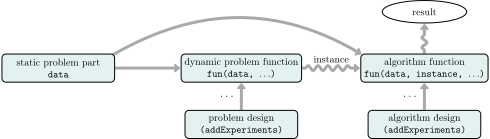
\includegraphics[width=1\textwidth,height=\textheight]{chapters/chapter11/Figures/mlr3book_figures-31.png}

}

\caption{\label{fig-batchtools-illustration}Illustration of a batchtools
problem, algorithm, and experiment.}

\end{figure}

Next, we need to specify the algorithm to run with
\href{https://www.rdocumentation.org/packages/batchtools/topics/addAlgorithm}{\texttt{addAlgorithm()}}.
Algorithms are again specified with a unique \texttt{name}, as well as a
function to define the computational steps of the experiment and to
return its result.

Here, we define one job to represent a complete resample experiment. In
general, algorithms in \texttt{batchtools} may return arbitrary objects
-- those are simply stored on the file system and can be processed with
a custom function while collecting the results.

\begin{Shaded}
\begin{Highlighting}[]
\FunctionTok{addAlgorithm}\NormalTok{(}
  \StringTok{"run\_learner"}\NormalTok{,}
  \AttributeTok{fun =} \ControlFlowTok{function}\NormalTok{(instance, learner, job, ...) \{}
    \FunctionTok{resample}\NormalTok{(instance}\SpecialCharTok{$}\NormalTok{task, learner, instance}\SpecialCharTok{$}\NormalTok{resampling)}
\NormalTok{  \},}
  \AttributeTok{reg =}\NormalTok{ reg}
\NormalTok{)}
\end{Highlighting}
\end{Shaded}

Finally, we will define concrete experiments with
\href{https://www.rdocumentation.org/packages/batchtools/topics/addExperiments}{\texttt{addExperiments()}}
by passing problem designs (\texttt{prob.designs}) and algorithm designs
(\texttt{algo.designs}) that assign parameters to problems and
algorithms, respectively (Figure~\ref{fig-batchtools-illustration}).

In the code below, we add all resampling iterations for the six tasks as
experiments. By leaving \texttt{prob.designs} unspecified, experiments
for all existing problems are created per default. We set the
\texttt{learner} parameter of our algorithm (\texttt{"run\_learner"}) to
be the three learners from our \texttt{large\_design} object. Note that
whenever an experiment is added, the current seed is assigned to the
experiment and then incremented.

\begin{Shaded}
\begin{Highlighting}[]
\NormalTok{alg\_des }\OtherTok{=} \FunctionTok{list}\NormalTok{(}\AttributeTok{run\_learner =} \FunctionTok{data.table}\NormalTok{(}\AttributeTok{learner =}\NormalTok{ learners))}
\FunctionTok{addExperiments}\NormalTok{(}\AttributeTok{algo.designs =}\NormalTok{ alg\_des, }\AttributeTok{reg =}\NormalTok{ reg)}
\FunctionTok{summarizeExperiments}\NormalTok{()}
\end{Highlighting}
\end{Shaded}

Our jobs can now be submitted to the cluster; by not specifying specific
job IDs, \emph{all} experiments are submitted.

\begin{Shaded}
\begin{Highlighting}[]
\FunctionTok{submitJobs}\NormalTok{(}\AttributeTok{reg =}\NormalTok{ reg)}
\end{Highlighting}
\end{Shaded}

We can retrieve the job results using
\href{https://www.rdocumentation.org/packages/batchtools/topics/loadResult}{\texttt{loadResult()}},
which outputs the objects returned by the algorithm function, which in
our case is a
\href{https://mlr3.mlr-org.com/reference/ResampleResult.html}{\texttt{ResampleResult}}.
To retrieve all results at once, we can use
\href{https://www.rdocumentation.org/packages/batchtools/topics/reduceResults}{\texttt{reduceResults()}}
to create a single
\href{https://mlr3.mlr-org.com/reference/BenchmarkResult.html}{\texttt{BenchmarkResult}}.
For this, we use the combine function \texttt{c()} which can combine
multiple objects of type \texttt{ResampleResult} or
\texttt{BenchmarkResult} to a single \texttt{BenchmarkResult}.

\begin{Shaded}
\begin{Highlighting}[]
\NormalTok{rr }\OtherTok{=} \FunctionTok{loadResult}\NormalTok{(}\DecValTok{1}\NormalTok{, }\AttributeTok{reg =}\NormalTok{ reg)}
\FunctionTok{as.data.table}\NormalTok{(rr)[}\DecValTok{1}\SpecialCharTok{:}\DecValTok{5}\NormalTok{]}
\end{Highlighting}
\end{Shaded}

\begin{verbatim}
                task            learner             resampling
1: <TaskClassif[51]> <GraphLearner[38]> <ResamplingCustom[20]>
2: <TaskClassif[51]> <GraphLearner[38]> <ResamplingCustom[20]>
3: <TaskClassif[51]> <GraphLearner[38]> <ResamplingCustom[20]>
4: <TaskClassif[51]> <GraphLearner[38]> <ResamplingCustom[20]>
5: <TaskClassif[51]> <GraphLearner[38]> <ResamplingCustom[20]>
2 variables not shown: [iteration, prediction]
\end{verbatim}

\begin{Shaded}
\begin{Highlighting}[]
\NormalTok{bmr }\OtherTok{=} \FunctionTok{reduceResults}\NormalTok{(c, }\AttributeTok{reg =}\NormalTok{ reg)}
\NormalTok{bmr}\SpecialCharTok{$}\FunctionTok{aggregate}\NormalTok{()[}\DecValTok{1}\SpecialCharTok{:}\DecValTok{5}\NormalTok{]}
\end{Highlighting}
\end{Shaded}

\begin{verbatim}
   nr  task_id  learner_id resampling_id iters classif.ce
1:  1 kr-vs-kp      logreg        custom    10    0.02566
2:  2 kr-vs-kp      ranger        custom    10    0.01377
3:  3 kr-vs-kp featureless        custom    10    0.47778
4:  4 breast-w      logreg        custom    10    0.03578
5:  5 breast-w      ranger        custom    10    0.02861
Hidden columns: resample_result
\end{verbatim}

\hypertarget{sec-benchmark-analysis}{%
\section{Statistical Analysis}\label{sec-benchmark-analysis}}

The final step of a benchmarking experiment is to use statistical tests
to determine which (if any) of our learners performed the best.
\href{https://mlr3benchmark.mlr-org.com/reference/mlr3benchmark-package.html}{\texttt{mlr3benchmark}}
provides infrastructure for applying statistical significance tests on
\href{https://mlr3.mlr-org.com/reference/BenchmarkResult.html}{\texttt{BenchmarkResult}}
objects.

Currently, Friedman\index{friedman} tests and pairwise Friedman-Nemenyi
tests (Demšar 2006) are supported to analyze benchmark experiments with
at least two independent tasks and at least two learners. As a first
step, we recommend performing a pairwise comparison of learners using
pairwise Friedman-Nemenyi tests with \texttt{\$friedman\_posthoc()}.
This method first performs a global comparison to see if any learner is
statistically better than another. To use these methods we first convert
the benchmark result to a
\href{https://mlr3benchmark.mlr-org.com/reference/BenchmarkAggr.html}{\texttt{BenchmarkAggr}}
object using
\href{https://mlr3benchmark.mlr-org.com/reference/as_benchmark_aggr.html}{\texttt{as\_benchmark\_aggr()}}\index{\texttt{as\_benchmark\_aggr()}}{\marginnote{\begin{footnotesize}\texttt{as\_benchmark\_aggr()}\end{footnotesize}}}.

\begin{Shaded}
\begin{Highlighting}[]
\FunctionTok{library}\NormalTok{(mlr3benchmark)}
\NormalTok{bma }\OtherTok{=} \FunctionTok{as\_benchmark\_aggr}\NormalTok{(bmr, }\AttributeTok{measures =} \FunctionTok{msr}\NormalTok{(}\StringTok{"classif.ce"}\NormalTok{))}
\NormalTok{bma}\SpecialCharTok{$}\FunctionTok{friedman\_posthoc}\NormalTok{()}
\end{Highlighting}
\end{Shaded}

\begin{verbatim}

    Pairwise comparisons using Nemenyi-Wilcoxon-Wilcox all-pairs test for a
    		two-way balanced complete block design
\end{verbatim}

\begin{verbatim}
data: ce and learner_id and task_id
\end{verbatim}

\begin{verbatim}
            logreg ranger
ranger      0.1932 -     
featureless 0.1932 0.0015
\end{verbatim}

\begin{verbatim}

P value adjustment method: single-step
\end{verbatim}

These results indicate a statistically significant difference between
the \texttt{"featureless"} learner and \texttt{"ranger"} (assuming
\(p\leq0.05\) is significant). This table can be visualized in a
critical difference plot (Figure~\ref{fig-lsb-cd}), which typically
shows the mean rank of a learning algorithm on the x-axis along with a
thick horizontal line that connects learners that are pairwise not
significantly different (while correcting for multiple tests).

\begin{Shaded}
\begin{Highlighting}[]
\FunctionTok{autoplot}\NormalTok{(bma, }\AttributeTok{type =} \StringTok{"cd"}\NormalTok{, }\AttributeTok{ratio =} \DecValTok{1}\SpecialCharTok{/}\DecValTok{5}\NormalTok{)}
\end{Highlighting}
\end{Shaded}

\begin{figure}[H]

{\centering \includegraphics[width=1\textwidth,height=\textheight]{chapters/chapter11/large-scale_benchmarking_files/figure-pdf/fig-lsb-cd-1.pdf}

}

\caption{\label{fig-lsb-cd}Critical difference diagram comparing the
random forest, logistic regression, and featureless baseline. The
critical difference of 1.35 in the title refers to the difference in
mean rank required to conclude that one learner performs statistically
different to another.}

\end{figure}

Using Figure~\ref{fig-lsb-cd} we can conclude that on average the random
forest had the lowest (i.e., best) rank, followed by the logistic
regression, and then the featureless baseline. While the random forest
was statistically better performing than the baseline (no connecting
line in Figure~\ref{fig-lsb-cd}), it was not statistically superior to
the logistic regression (connecting line in Figure~\ref{fig-lsb-cd}). We
could now further compare this with the large benchmark study conducted
by Couronné, Probst, and Boulesteix (2018), where the random forest
outperformed the logistic regression in 69\% of 243 real-world datasets.

\hypertarget{conclusion-9}{%
\section{Conclusion}\label{conclusion-9}}

In this chapter, we have explored how to conduct large-scale machine
learning experiments using \texttt{mlr3}. We have shown how to acquire
diverse datasets from OpenML through the
\href{https://mlr3oml.mlr-org.com}{\texttt{mlr3oml}}\index{\texttt{mlr3oml}}
interface package, how to execute large-scale experiments with
\texttt{batchtools} and
\href{https://mlr3batchmark.mlr-org.com}{\texttt{mlr3batchmark}}\index{\texttt{mlr3batchmark}}
integration, and finally how to analyze the results of these experiments
with
\href{https://mlr3benchmark.mlr-org.com}{\texttt{mlr3benchmark}}\index{\texttt{mlr3benchmark}}.
For further reading about
\href{https://cran.r-project.org/package=batchtools}{\texttt{batchtools}}
we recommend Lang, Bischl, and Surmann (2017) and Bischl et al. (2015).

\hypertarget{tbl-api-large-benchmarking}{}
\begin{longtable}[]{@{}
  >{\raggedright\arraybackslash}p{(\columnwidth - 4\tabcolsep) * \real{0.3333}}
  >{\raggedright\arraybackslash}p{(\columnwidth - 4\tabcolsep) * \real{0.3333}}
  >{\raggedright\arraybackslash}p{(\columnwidth - 4\tabcolsep) * \real{0.3333}}@{}}
\caption{\label{tbl-api-large-benchmarking}Important classes and
functions covered in this chapter with underlying class (if applicable),
class constructor or function, and important class fields and methods
(if applicable).}\tabularnewline
\toprule\noalign{}
\begin{minipage}[b]{\linewidth}\raggedright
Class
\end{minipage} & \begin{minipage}[b]{\linewidth}\raggedright
Constructor/Function
\end{minipage} & \begin{minipage}[b]{\linewidth}\raggedright
Fields/Methods
\end{minipage} \\
\midrule\noalign{}
\endfirsthead
\toprule\noalign{}
\begin{minipage}[b]{\linewidth}\raggedright
Class
\end{minipage} & \begin{minipage}[b]{\linewidth}\raggedright
Constructor/Function
\end{minipage} & \begin{minipage}[b]{\linewidth}\raggedright
Fields/Methods
\end{minipage} \\
\midrule\noalign{}
\endhead
\bottomrule\noalign{}
\endlastfoot
\href{https://mlr3oml.mlr-org.com/reference/oml_data.html}{\texttt{OMLData}}
&
\href{https://mlr3oml.mlr-org.com/reference/oml_sugar.html}{\texttt{odt()}}
& \texttt{\$data}; \texttt{\$feature\_names} \\
\href{https://mlr3oml.mlr-org.com/reference/oml_task.html}{\texttt{OMLTask}}
&
\href{https://mlr3oml.mlr-org.com/reference/oml_sugar.html}{\texttt{otsk()}}
& \texttt{\$data}; \texttt{\$task\_splits} \\
\href{https://mlr3oml.mlr-org.com/reference/oml_collection.html}{\texttt{OMLCollection}}
&
\href{https://mlr3oml.mlr-org.com/reference/oml_sugar.html}{\texttt{ocl()}}
& \texttt{\$task\_ids} \\
\texttt{Registry} &
\href{https://www.rdocumentation.org/packages/batchtools/topics/makeExperimentRegistry}{\texttt{makeExperimentRegistry()}}
&
\href{https://www.rdocumentation.org/packages/batchtools/topics/submitJobs}{\texttt{submitJobs()}};
\href{https://www.rdocumentation.org/packages/batchtools/topics/getStatus}{\texttt{getStatus()}};
\href{https://mlr3batchmark.mlr-org.com/reference/reduceResultsBatchmark.html}{\texttt{reduceResultsBatchmark}};
\href{https://www.rdocumentation.org/packages/batchtools/topics/getJobTable}{\texttt{getJobTable}} \\
&
\href{https://mlr3batchmark.mlr-org.com/reference/batchmark.html}{\texttt{batchmark()}}
& - \\
\href{https://mlr3benchmark.mlr-org.com/reference/BenchmarkAggr.html}{\texttt{BenchmarkAggr()}}
&
\href{https://mlr3benchmark.mlr-org.com/reference/as_benchmark_aggr.html}{\texttt{as\_benchmark\_aggr()}}
& \texttt{\$friedman\_posthoc()} \\
\end{longtable}

\hypertarget{exercises-9}{%
\section{Exercises}\label{exercises-9}}

In these exercises, we will conduct an empirical study analyzing whether
a random forest is predictively stronger than a single decision tree.
Our null hypothesis is that there is no significant performance
difference.

\begin{enumerate}
\def\labelenumi{\arabic{enumi}.}
\tightlist
\item
  Load the OpenML collection with ID 269, which contains regression
  tasks from the AutoML benchmark (Gijsbers et al. 2022). Peek into this
  suite to study the contained data sets and their characteristics. Then
  find all tasks with less than 4000 observations and convert them to
  \texttt{mlr3} tasks.
\item
  Create an experimental design that compares
  \texttt{lrn("regr.ranger")} and \texttt{lrn("regr.rpart")} on those
  tasks. Use the robustify pipeline for both learners and a featureless
  fallback learner. You can use three-fold CV instead of the OpenML
  resamplings to save time. Run the comparison experiments with
  \texttt{batchtools}. Use default hyperparameter settings and do not
  perform any tuning to keep the experiments simple.
\item
  Conduct a global Friedman test and, if appropriate, post hoc
  Friedman-Nemenyi tests, and interpret the results. As an evaluation
  measure, use the MSE.
\end{enumerate}
